\begin{frame}{Resultados experimento}
	EXPLICA ERRO DA DISSERTACAO
\end{frame}

\begin{frame}{Resultados experimento}
Com a possibilidade da modulação de carga, é possível verificar o impacto da carga modulada no ambiente projetado para o trabalho de Mamani (2015). 
	\begin{itemize}
		\item inicialmente utilizado 40\% da carga até o instante de 30 segundos de experimentação
	
		\item a partir de 30 segundos um crescimento brusco na carga utilizando os 60\% restante da carga, e gerando um degrau positivo. A carga mantém-se máxima, em 100\%, durante 40 segundos 
	
		\item apos decorridos 70 segundo de experimentação), a uma queda súbita voltando a trabalhar com 40\% da carga até o final do experimento.
	\end{itemize}
\end{frame}

\begin{frame}{Conexões por segundo vs Tempo de resposta}
	\begin{figure}[htb]
		\centering
		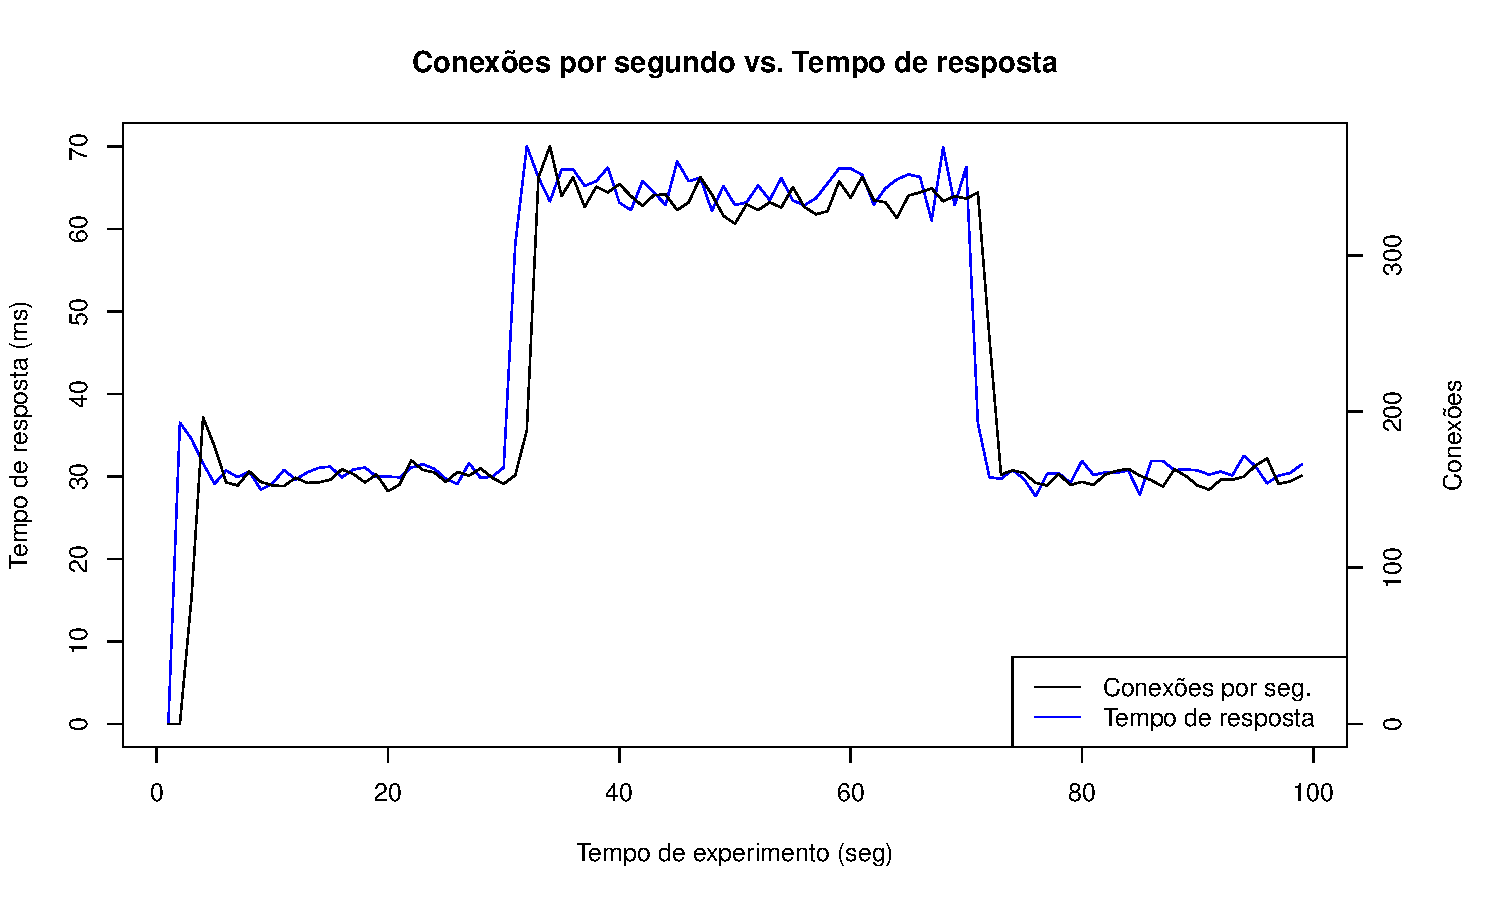
\includegraphics[scale=0.5]{../monograph/images/cps-resp60.pdf}	
		\label{fig:cps-resp60}
	\end{figure}
\end{frame}

\begin{frame}{Conexões por segundo vs Média de utilização das CPU VMs}
	\begin{figure}[htb]
		\centering
		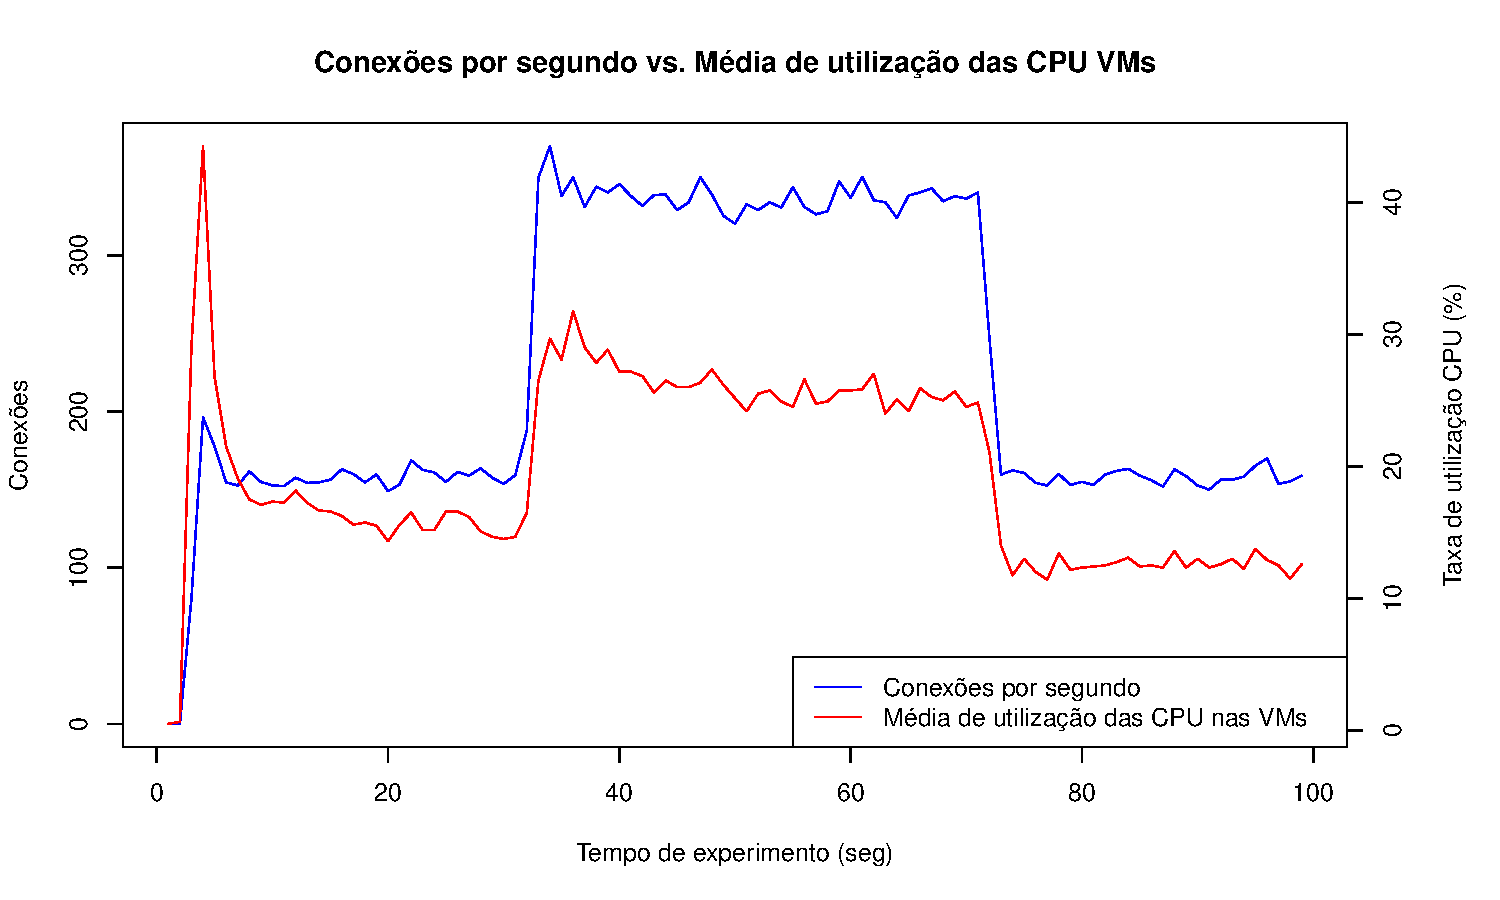
\includegraphics[scale=0.5]{../monograph/images/cps-vmcpu60.pdf}
		\label{fig:cps-vmcpu60}
	\end{figure}
\end{frame}

\begin{frame}{Conexões por segundo vs Utilização de CPU Banco de dados}
	\begin{figure}[htb]
		\centering
		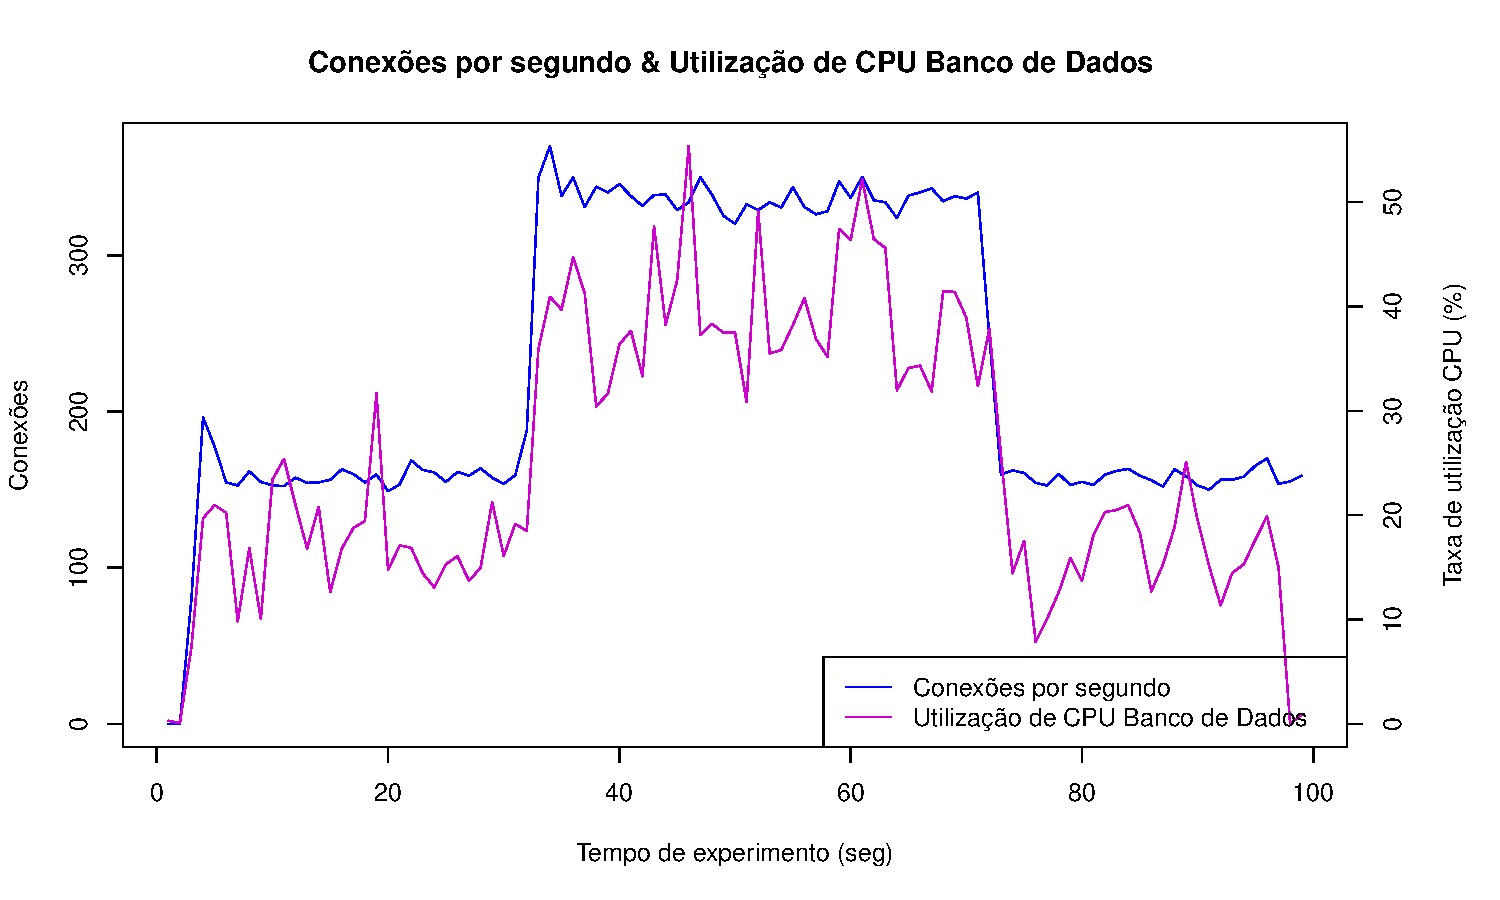
\includegraphics[scale=0.5]{../monograph/images/cps-dbcpu60.pdf}
		\label{fig:cps-dbcpu60}
	\end{figure}
\end{frame}

\begin{frame}{Tempo de resposta VS Utilização de CPU Banco de dados}
	\begin{figure}[htb]
		\centering
		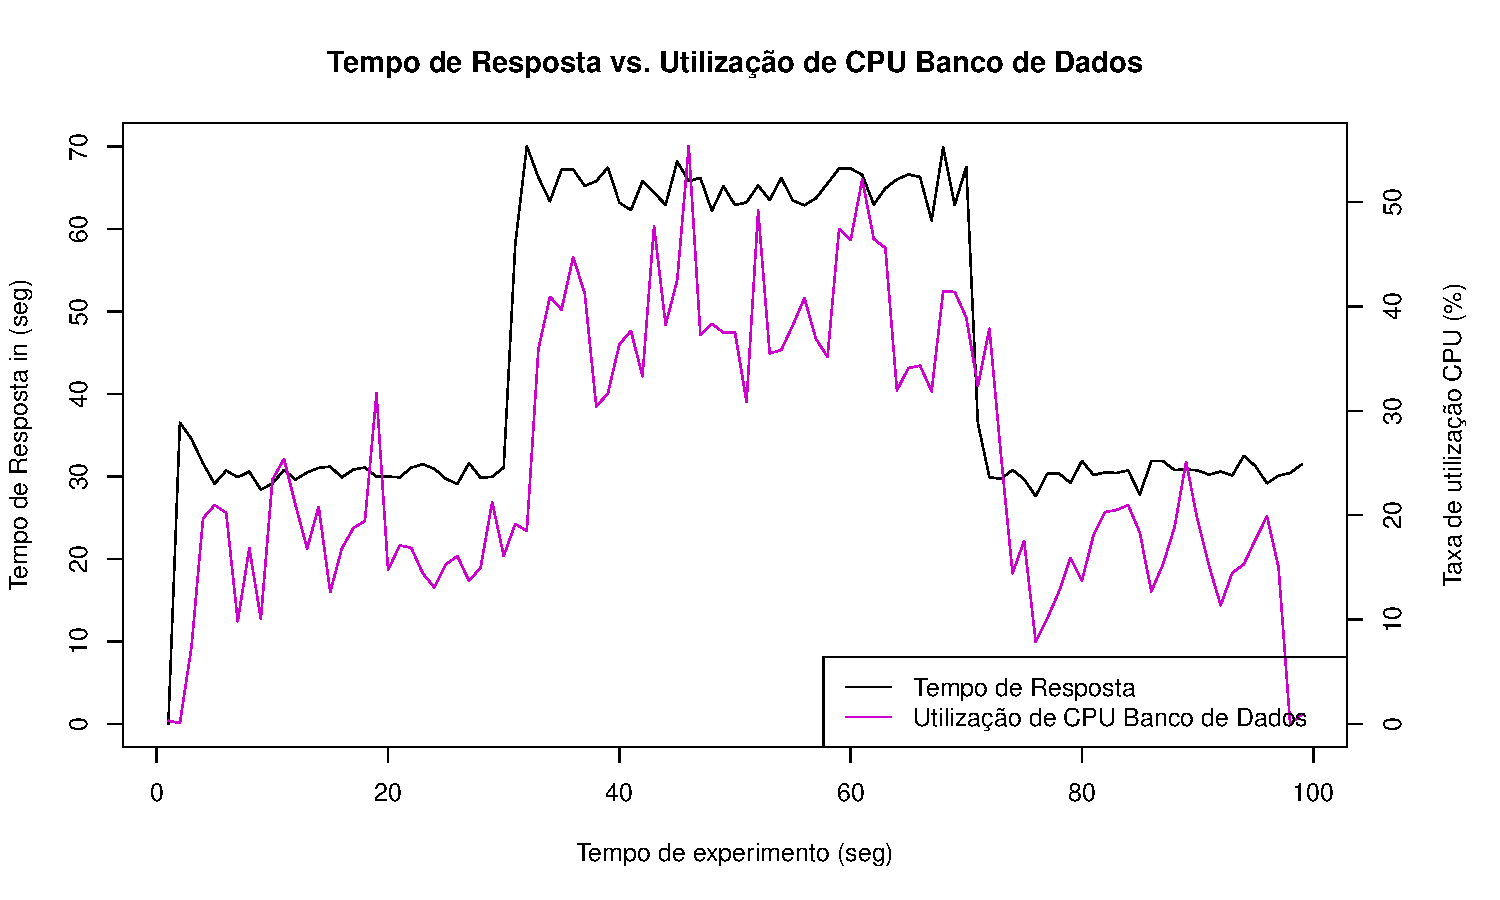
\includegraphics[scale=0.5]{../monograph/images/resp-dbcpu60.pdf}
		\label{fig:resp-dbcpu60}
	\end{figure}
\end{frame}



